\chapter{Hardware Evaluation}
\label{ch:hardware}
This chapter starts with a brief introduction of the sensor employed in this thesis(sec. \ref{sec:imcr}).
The system properties and specifications are outlined, and the makeup of the antenna array is described.
On the basis of this knowledge, the system can be evaluated through a number of experiments.

The second part of this chapter (sec. \ref{sec:stability_analysis}) focuses on stability analysis,
which is conducted through long-term static measurements of a corner reflector.
By monitoring the radar system's performance over an extended period,
we aim to assess its stability and reliability in real-world operating conditions.
The analysis provides insights into any temporal variations or drifts in system parameters,
enabling proactive measures to mitigate potential sources of error.

The third part of this chapter (sec. \ref{sec:calibration}) focuses on antenna gain measurements using a rotating setup.
Antenna gain plays a crucial role in radar imaging, affecting the system's sensitivity and resolution.
By rotating the radar system and precisely measuring the received signals from known targets,
we can accurately determine the antenna gain across different azimuth angles.
This measurement process enables the characterization and validation of antenna performance,
facilitating improved imaging accuracy and consistency. \\

Through these procedures, Chapter 3 aims to establish a robust foundation
for the subsequent imaging algorithms that are implemented and evaluated in Chapter 4.
By ensuring the stability of system parameters and accurately characterizing antenna performance,
we strive to enhance the reliability and effectiveness of FMCW MIMO radar imaging for various applications.

\begin{figure}
    \centering
    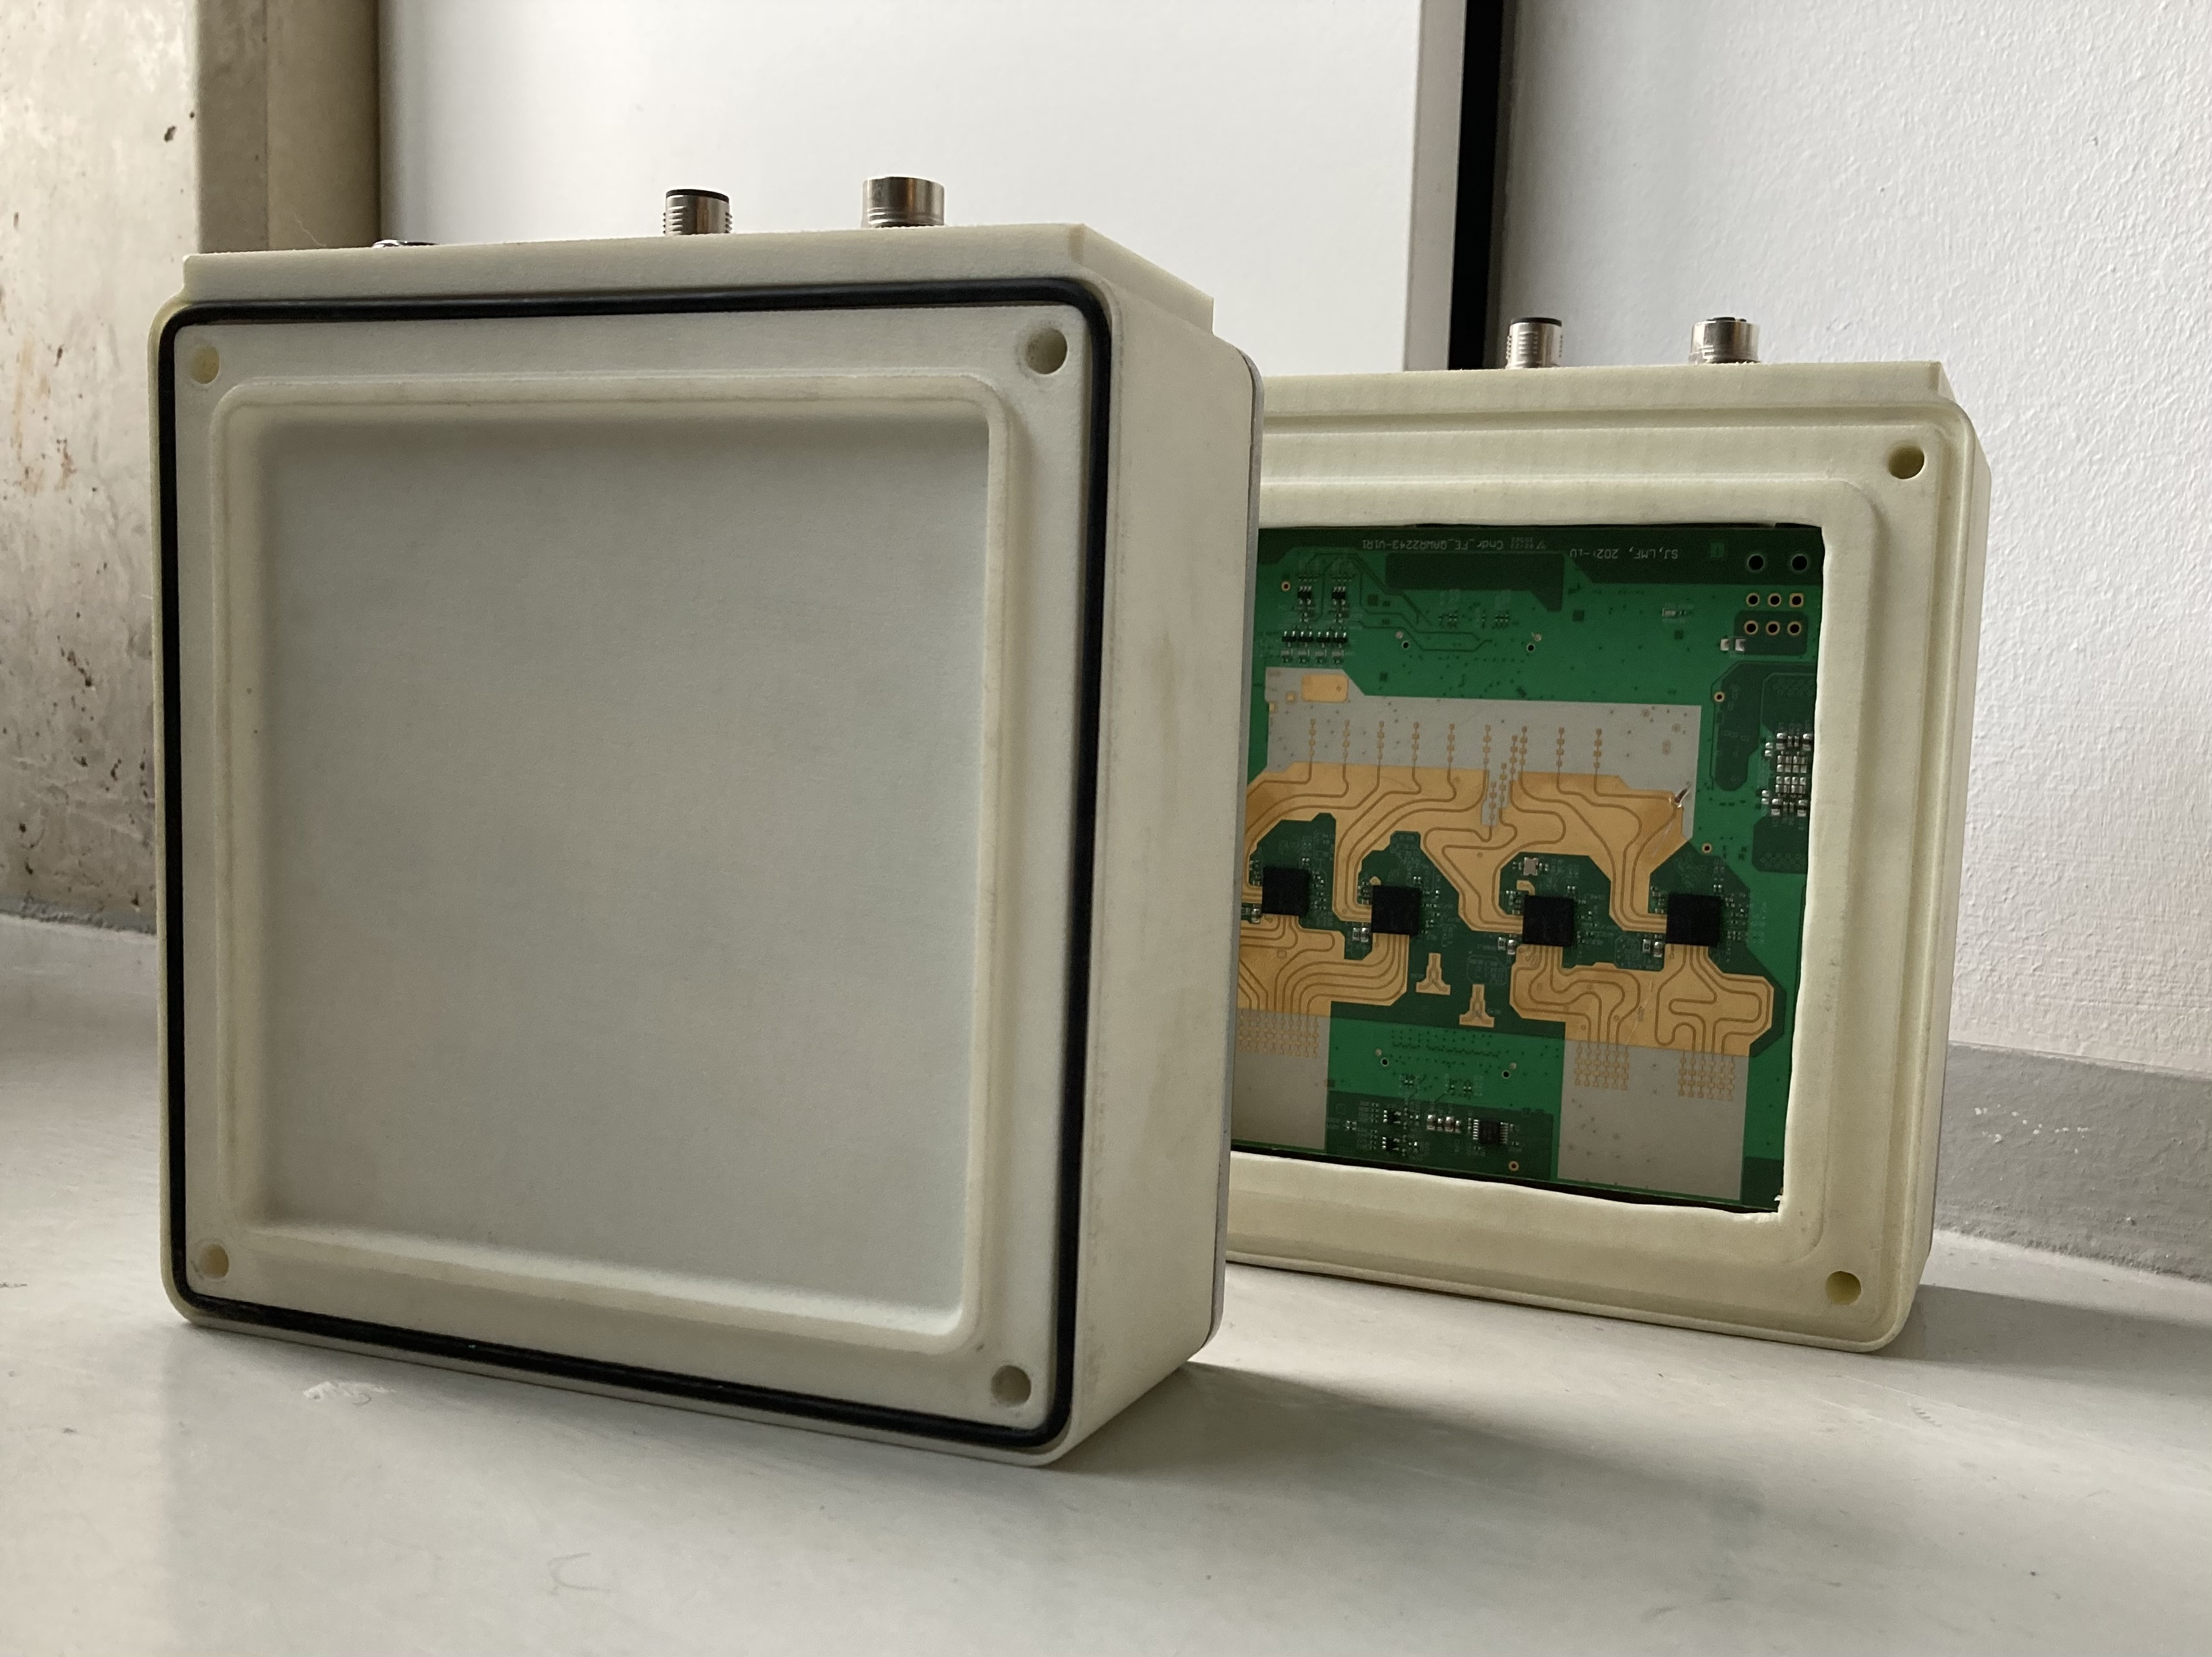
\includegraphics[width=0.6\textwidth]{../figures/imcr.jpg}
    \caption{The iMCR Sensor. closed housing (left) and open housing (right)}
    \label{fig:imcr}
\end{figure}

\section{Indurad Multi-Channel Radar}
\label{sec:imcr}
The sensor employed in this thesis operates on Multiple Input Multiple Output (MIMO) Frequency Modulated Continuous Wave (FMCW) technology,
showcasing advanced features tailored for precise radar imaging.

- applications

\subsection{Sytem Parameters}

\cref{tab:imcr} summarizes the key technical characteristics of the sensor.
The iMCR offers a range capability of up to 100 meters, extendable to 800 meters with active beamforming techniques.
The sensor achieves a remarkable range resolution of \SI{3.8}{\mm}, enabling detailed imaging of objects within its detection range.
Utilizing a sawtooth or chirp signal type, the sensor employs Time Division Multiplexing (TDM) in transmission for efficient multiplexing.
Operating within the frequency range of \SIrange{77}{81}{\GHz},
it leverages the millimeter-wave spectrum to achieve high-resolution imaging suitable for a variety of applications.
The chirp duration of the sensor is between about \SIrange{60}{70}{\GHz}, ensuring effective signal processing and data acquisition.
Equipped with 12 transmit antennas and 16 receive antennas, the sensor offers comprehensive coverage and sensitivity,
facilitating robust imaging performance.
Furthermore, the sensor's Intermediate Frequency (IF) samplerate is set at \SI{22}{\MHz},
providing sufficient bandwidth for accurate signal processing and analysis.
This combination of advanced features and specifications positions the sensor as a versatile and effective tool for radar imaging tasks in diverse scenarios,
ranging from automotive safety systems to industrial sensing applications. \\

\begin{table}[h]
    \centering
    \begin{tabular}{ll}
        \toprule
        \textbf{Radar Characteristic} & \textbf{iMCR  }                                     \\
        \midrule
        Technology                    & mmWave FMCW MIMO                                    \\
        Maximum Range                 & \SI{100}{\m} (\SI{800}{\m} with active beamforming) \\
        Range Resolution              & \SI{3.8}{\mm}                                       \\
        FM Type                       & Sawtooth/Chirp                                      \\
        Multiplexing                  & TDM in Tx                                           \\
        Frequency                     & \SIrange{77}{81}{\GHz}                              \\
        Chirp Duration                & \SIrange{60}{70}{\us}                               \\
        Antennas                      & 12 Tx, 16 Rx                                        \\
        IF Samplerate                 & \SI{22}{\MHz}                                       \\
        \bottomrule
    \end{tabular}
    \caption{iMCR: Technical Overview}
    \label{tab:imcr}
\end{table}

\cref{fig:imcr} shows the sensor in a watertight closed housing,
and an open housing. The closed housing is ideal for mining applications,
but for development purposes, the open housing may be preferable since it has a no impact on the input signals.

The sytem can be subdivided into a frontend and a backend.
The frontend consists of the antennas, and the transmitter and receivers.
The transmitters and receivers are implemented through a cascaded setup
of four Texas Instruments\textregistered AWR2243P\texttrademark chips.

The backend enables integration of the sensor into imaging applications.
It consists of an FPGA that is used for receiving data from the frontend
and its configuration, and a computer running an embedded Linux system.
The software running on this system operates the FPGA and
sends the received radar data through TCP.

\subsection{Virtual Antenna Array}

As described in \cref{sec:virtual_array},
a virtual antenna array is the far-field equivalent SIMO array that can be derived for a given MIMO array.
It is also a useful tool to gain an intuition on the resolution capabilities of an array.
\\

\cref{fig:imcr_antpos} shows the physical positions of the transmit and receive array.
The transmit array consist of four groups of three antennas.
Apart from one group, they are evenly spaced horizontal at the same height, with a distance of $4d=2\lambda_0$ between the members of a group.
The exception is made by the antennas driven by chip 1, which are located at different heights.
The receive array consists of four groups physically separated of four antennas that are spaced exactly $d=\lambda_0/2$ apart horizontally.
They are all at the same height.

\cref{fig:imcr_virt_array} shows the corresponding virtual array.
Due to the distribution of antennas in the physical array, all antennas in the virtual array fall exactly onto a grid with $\lambda_0/2$.
The majority of the virtual antennas is located at the same height.
Indeed, some elements in the virtual array even overlap.
In the following, these elements will be referred to as the \emph{azimuth array}.
The remaining elements are are at different heights,
and will be referred to as the \emph{elevation channels}.
\begin{figure}
    \centering
    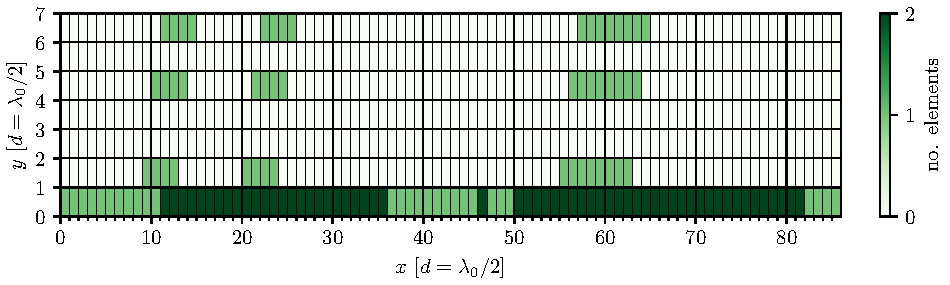
\includegraphics[width=\textwidth]{../figures/virt_array.pdf}
    \caption{iMCR virtual array}
    \label{fig:imcr_virt_array}
\end{figure}

\begin{figure}
    \centering
    \includegraphics[width=\textwidth]{../figures/imcr_antpos.pdf}
    \caption{iMCR transmit and receive antenna positions}
    \label{fig:imcr_antpos}
\end{figure}

